\section{The Compact Muon Solenoid}
At one of the collision points of the LHC, the CMS detector\cite{CMS, Bayatian:2006zz,Bayatian:922757} is placed. Weighing 14 000 \si{ \tonne}, This cylindrical detector is about 28.7 \si{ \meter} long and 15 \si{ \meter} in diameter, weighing around 14 000 \si{ \tonne}. It has an onion like structure of several specialised detectors and contains a superconducting solenoid with a magnetic field of 3.8 \si{ \Tesla}. The CMS detector is designed in a way that it can address the needs of physics coming from the LHC. Living in a hadronic environment, multi-jet processes produced by the strong interaction are a main source of background for rare physics processes. Therefore, good identification, momentum resolution, and charge determination of muon, electrons and photons is one of the main goals of the CMS detector. Further it provides a good charged particle momentum resolution and reconstruction efficiency in the inner tracker such that for example jets coming from b quarks or tau particles can be identified. Also th electromagnetic resolution for an efficient photon and lepton isolation as well as a good hadronic calorimeter for the missing transverse energy were kept into account while designing CMS. 

The LHC provides many collisions in a short amount of time. In order to discriminate between consecutive collisions - known as out of time pile up events - , CMS has to complete the full data acquisition for one collision event before the next one happen (around 50 \si{ \nano \second} (FIXME) ). Furthermore, since the photons are in packets, around 21 (FIXME) inelastic collisions happen every beam crossing. This creates a great amount of background processes in the detector called in time pile up events. Due to this difficult conditions, the detector has a great granularity which on its turn creates a need for huge number of synchronized electronic channels. Furthermore, due to to high flux of particles in the regions close to the beam, the electronics has to be able to endure high radiation. 


Before the start of taking collision data for 13 \si{ \TeV} operations on 3 June, CMS had a long shutdown. During this shut down several upgrades were performed:
\begin{itemize}
	\item Data Acquisition: new architercture, hardware and software
	\item Trigger Control and Distribution System: new uTCA
	\item Level-1 Trigger: new calorimeter trigger (uTCA)
	\item Electromagnetic calorimeter: new trigger optical links
	\item Hadronic calorimeter: new SiPMS (HO), new PMTs (HF), HF backend (uTCA)
	\item Drift tube chambers: new trigger electronics
	\item Resistive plate chambers: new chambers
	\item Cathode Strip Chamber: bew chambers and electronics
	\item Silicon pixel: lower temperature (-10 degrees) and recovered channels
	\item Silicon tracker: lower temperature (-15 degrees)
	\item Luminosity and beam monitoring: new pixel luminosity telescope, fact beams conditions monitor and beam halo monitor, bril-daq software 
\end{itemize}


\subsection{CMS coordinate system}
The coordinate system used by CMS can be found in Figure~\ref{fig:CMScoord}. The origin of the right handed orthogonal coordinate system is chosen to be the point of collisions. The x-axis points towards the centre of the LHC ring such that the y-axis points towards the sky, and the z-axis lies tangent to the beam axis. Since the experiment has a cylindrical shape, customary coordinates are used to describe the momentum \impuls: the distance $\rho$, the azimuthal angle $\phi \in \left[-\pi,\pi\right]$ - the angle between the x-axis and the projection in the transverse plane of \impuls (\trimpuls) - , the pseudo-rapidity \psrap - expressed by the polar angle $\theta$ between the direction of \impuls and the beam - : 
\begin{equation}
\eta = - \ln \left(\tan \left(\frac{\theta}{2}\right)\right).
\end{equation}
For the energies considered at the LHC, where $E >> m$, the pseudo-rapidity is a good approximation of the rapidity $y$
\begin{equation}
y = \frac{1}{2} \ln \left(\frac{E + p_z}{E - p_z}\right), 
\end{equation}
where the difference of rapidities of two particles is invariant under a Lorentz boost in the z-direction.
 \begin{figure}[ht]
	\centering
	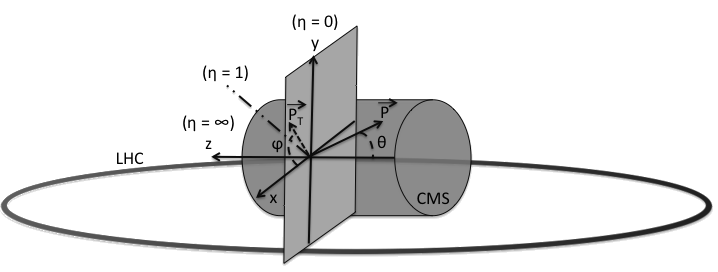
\includegraphics[width=0.75\textwidth]{2_ExperimentalSetup/Figures/imageedit_1_9146672677}
	\caption{Representation of the coordinate system used by CMS. The point of origin is put at the collision point. The x-axis points towards the centre of the LHC ring such that the z-axis lies tangent to the beam axis. }
	\label{fig:CMScoord}
\end{figure}

\subsection{Towards the heart of CMS}
The CMS detector consists of two parts; a central barrel around the beam pipe (\abspsrap $<1.4$) and two plugs to ensure the hermeticity of the detector. In Figure~\ref{fig:CMS} the onion like structure of the CMS detector is visible. The choice of a solenoid of 12.9 \si{ \meter} (FIXME) long and 5.9 \si{ \meter}
diameter gives the advantage of bending the particle trajectories in the transverse plane. The hadronic calorimeter,  the electromagnetic calorimeter and the tracker are within the solenoid, while the muon chambers are placed outside the solenoid.

\begin{figure}[ht]
   \centering
	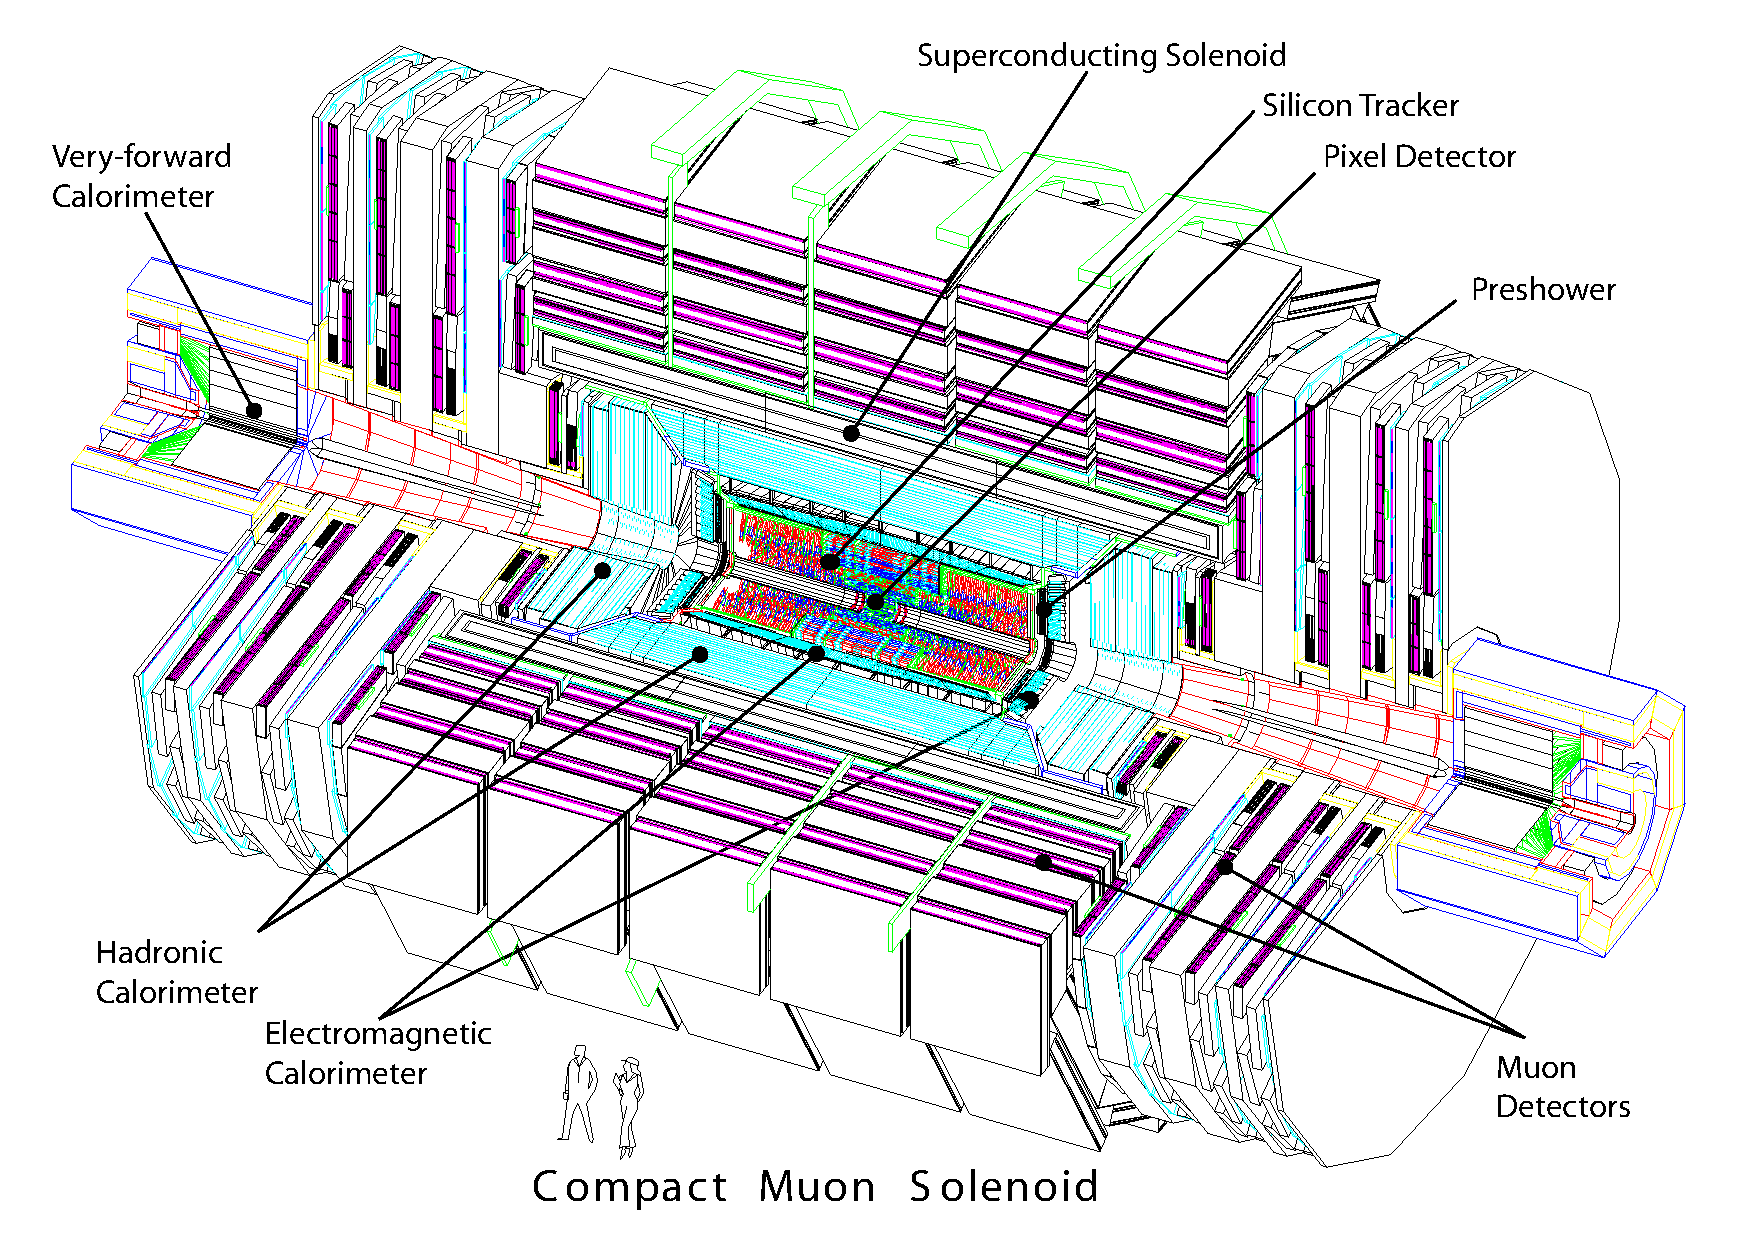
\includegraphics[width=\textwidth]{2_ExperimentalSetup/Figures/cms_complete_labelled}
	\caption{Mechanical layout of the CMS detector\cite{CMSdraw}.}
	\label{fig:CMS}
\end{figure}

	\subsubsection{Muon system}
	\subsubsection{Hadronic calorimeter}	
\subsubsection{Electromagnetic calorimeter}
The electromagnetic calorimeter (ECAL) is designed to measure the energy of photons and electrons and covers \abspsrap $<3$. It consists of 75 848 lead tungstae (PbW$O_4$) crystals. Electromagnetic showers produced by passing electrons or photons ionize the crystal atoms which emit a blue-green scintillation light, that is collected by silicon avalanche photodiodes (APDs) and vacuum phototriodes (VPTs). There are three regions: a central barrel (EB), a endcap region (EE) and a preshower (ES) (Figure \ref{fig:ECAL}). 
\begin{figure}[ht]
	\centering
	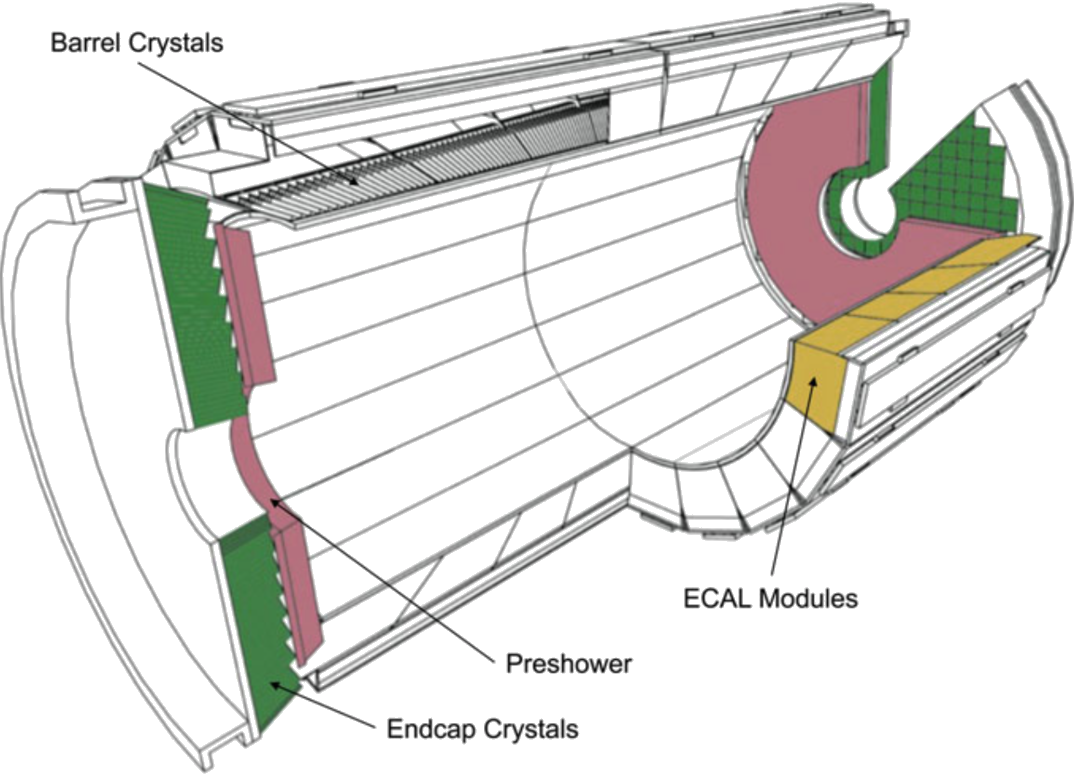
\includegraphics[width=0.75\textwidth]{2_ExperimentalSetup/Figures/imageedit_5_8264930617}
	\caption{Schematic cross section of the electromagnetic calorimeter\cite{Chatrchyan:2008aa}.}
	\label{fig:ECAL}
\end{figure}
The relative energy resolution of the ECAL for electrons is between 1.4-3\% in EB and 3-4\% for EE. In Figure \ref{fig:ECALres}, the resolutions for low and high bremsstrahlung electrons are shown. 
\begin{figure}[ht]
	\centering
	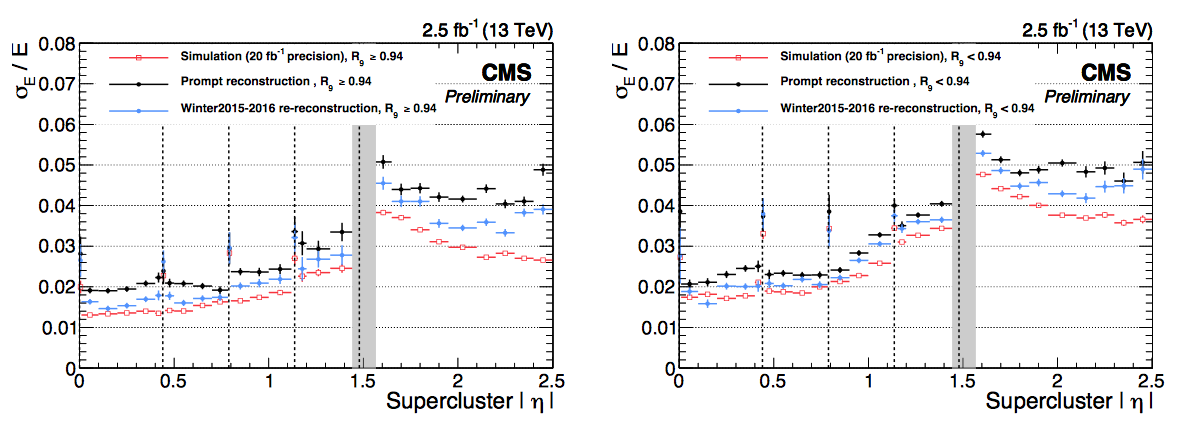
\includegraphics[width=\textwidth]{2_ExperimentalSetup/Figures/imageedit_7_5931623976}
	\caption{Relative energy resolution in bins of pseudo rapidity for the barrel and end caps using electrons from $Z \rightarrow ee$. Left: low bremsstrahlung electrons, Right: high brehmstrahlung electrons\cite{Sun:2233637}.}
	\label{fig:ECALres}
\end{figure}


\subsubsection{Inner tracking system and operations}
%https://indico.cern.ch/event/632928/
%http://cds.cern.ch/search?ln=en&cc=CMS+Reports&sc=1&p=tracker&f=title&action_search=Search
The tracking system (tracker)~\cite{Chatrchyan:1704291} is the detecting unit closest to the point of interaction. Responsible for the reconstruction of  trajectories from charged particles with \abspsrap $<2.5$, being bend by the magnetic field, it provides a measurement of the momentum. The tracker is also responsible for the determination of the interaction point or vertex. It should be able to provide high granularity as well as speed, and be able to endure high radiation. For this reason, the CMS collaboration choose silicon detector technology.

\begin{figure}[ht]
	\centering
%	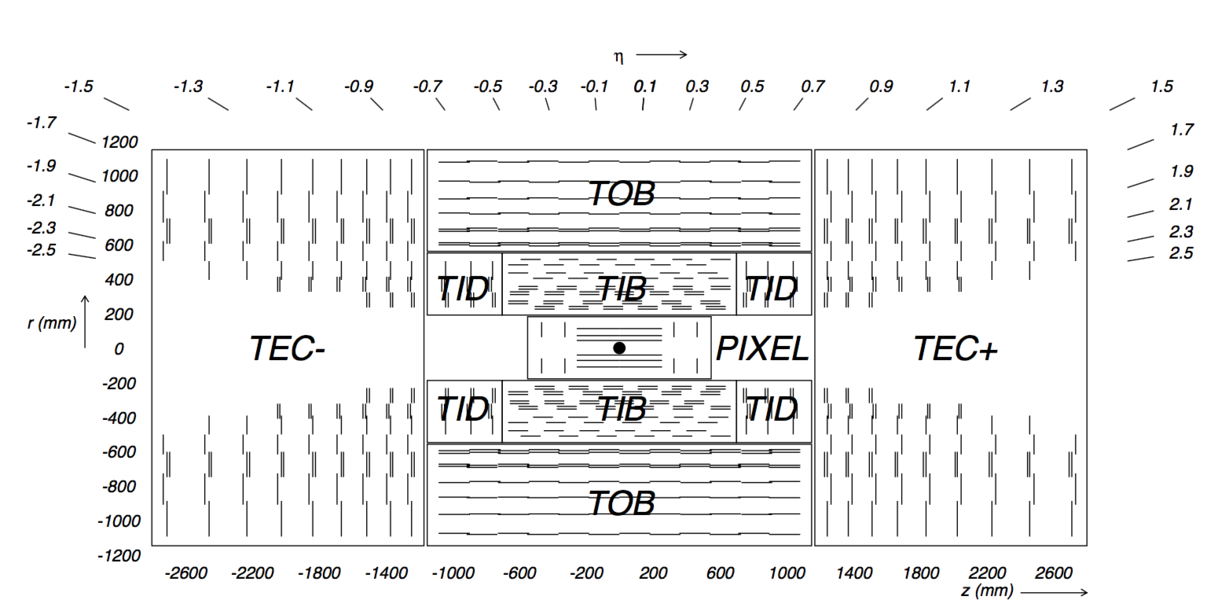
\includegraphics[width=\textwidth]{2_ExperimentalSetup/Figures/imageedit_3_5170744545}
	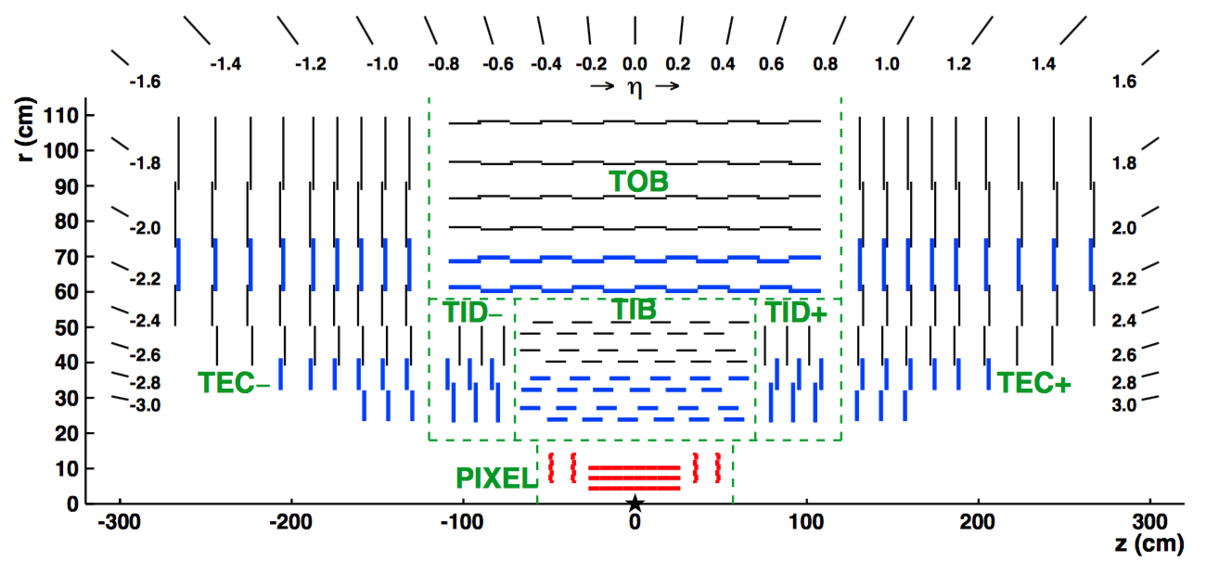
\includegraphics[width=\textwidth]{2_ExperimentalSetup/Figures/imageedit_11_9317262269}
%	\caption{Schematic cross section thorugh the CMS tracker. Each line represents a detector module. Double lines indicate back-to-back modules\cite{Chatrchyan:2008aa}.}
  \caption{Schematic cross section of the top galf of the CMS tracking system in the $rz$ plane. The centre of tracker is shown with a star and corresponds to the approximate position of the proton collision point. The green dashed lines are an indication for each named tracker subsystem. The strip tracker modules that provide two-dimensional hits are shown by thin, black lines, while those able to reconstruct three-dimensional hit positions are shown by thick, blue lines. The pixel modules, shown in red, also provide three-dimensional hits.  }
	\label{fig:Tracker}
\end{figure}

 The tracking system consists of a cylinder of 5.8 \si{ \meter} long and 2.5 \si{ \meter} in diameter. It is immersed in a co-axial magnetic field of 3.8 \si{ \Tesla} due to the solenoid.
 As shown Figure~\ref{fig:Tracker}, the tracker is built up from a large silicon strip tracker with a small silicon pixel inside. 
 The inner region, pixel ($4.4<r<10.2$ \si{ \cm}), gets the highest flux of particles. Therefore, pixel silicon sensors of $100 \times 150$ \si{ \squared \micro \meter} is used. It consists of three cylindrical barrels that are complemented by two discs of pixel modules at each side.
 The silicon strip tracker ($20<r<116$ \si{ \cm} ) has three subdivisions. The Tracker Inner Barrel  and Discs (TIB, TID) are composed of four barrel layers accompanied by three discs at each end. The outer part of the tracker - Tracker Outer Barrel (TOB) -  consists  of 6 barrel layers. In the outer discs, there are nine discs of silicon sensors, referred to as Tracker End Caps (TEC). 
  
 
 The pixel has 1440 modules that cover an area of about 1 \si{ \squared \meter} and have 66 million pixels. It provides a three-dimensional position measurement of the hits arising from the interaction from charged particles with the sensors. In transverse coordinate ($r\phi$), the hit position resolution is about 10 \si{ \micro \meter}, while 20-40 \si{ \micro \meter} is obtained in the longitudinal coordinate ($z$). The sensor plane position provides the third coordinate. 
  The silicon strip trackers consists of 15 148 single sided modules placed in the TIB, TID and the first four rings of the TEC. They provide 9.3 million readout channels. In the TOB and the outer three rings of the TEC, double sided modules are used. These modules are constructed from two back-to-back single sided modules, where one module is rotated through a stereo angle.  This covers an active area of about 198 \si{ \squared  \meter}. The TIB and TID provide position measurements in $r\phi$ with a resolution of approximately 13-38 \si{ \micro \meter}, while the TOB provides a resolution of about 18-47 \si{ \micro \meter}. The resolution in the  $z$ direction is approximately 230  \si{ \micro \meter} in the TIB/TID and 530  \si{ \micro \meter} in the TOB. To allow overlay and avoid gaps in acceptance, each module is shifted slightly in $r$ or $z$ with respect to its neighbouring modules within a layer. The resolution on the transverse momentum for a 100 \si{ \GeV} charged particle is abou 2.0\% (FIXME), while the impact parameter resolution is about 15 \si{ \micro \meter}. With this detector lay out, at least nine points per charged particle trajectory can be measured in an \abspsrap range up to 2.4.
  
   During the first data taking period of the LHC (2010 to 2013), the tracker operated at +4\si{ \degree C}. With the higher LHC beam intensities from 2015 onwards, the tracker needs to be operated at much lower temperatures. This is due to the fact with intense irradiation, the doping concentration changes, the leakage current increases proportional to the fluence and the charge collection efficiency decreases due to charge trapping. Mostly the leakage current (I) is affected by the temperature change: 
   \begin{equation}
   I \propto T^2 e^{-\frac{E_g}{2kT}}, 
   \end{equation}
    where $T$ is the operating temperature, $E_g$ the band gap and $k$ the Boltzmann constant. There is approximatly a factor 15 between the leakage currents at room temperatures and at $-10$ \si{ \degree C}. 
    % see http://www.hephy.at/user/friedl/diss/html/node14.html
    
    During the first long shutdown (LS1), the CMS cooling plant was refurbished\cite{running:1998606} and the fluorocarbon cooling system overhauled. To help to suppress the humidity inside the tracker, new methods for vapour sealing and insulation were applied. Furthermore, several hundred high-precision sensors are used to monitor the humidity and temperature. In order to get as dry air as possible, a new dry-gas plant provides eight times more dry gas (air or nitrogen) than during the first run, and allows regulation if the flow. As final addition, the cooling bundels outside the tracker are equipped with heater wires and temperature sensors in order to maintain safe operations. For the data taking in 2015-2016, the tracker operated at $-15$\si{ \degree C}.

\paragraph{Track reconstruction}
\paragraph{Primary vertex reconstruction}
\subsection{Data acquisition}
\subsection{CMS computing model}
%CMS trigger system 
% https://arxiv.org/abs/1609.02366